\section{Theoretical Analysis}
\label{sec:analysis}

We used the ideal diode model for the theoretical predictions, with a voltage $V_{on}=0.7V$. The reference values for $I_S$, $\eta$ and $V_T$ were taken from Ngspice's data from the Default Diode Model used by us.

\subsection{Envelope Detector Output Prediction}
\label{ed}

The theoretical calculations for the Envelope Detector circuit were based on the following model, considering that the beggining of each period is when $v_S$ (the Envelope Detector's input voltage) is at its maximum. \par

While $t<t_{off}$,
\begin{equation}
v_O=v_S
\label{eq:kvl3}
\end{equation}

 $t_{off}$ is given as 
\begin{equation}
\frac{1}{\omega}arctan(\frac{1}{\omega RC})
\label{eq:kvl4}
\end{equation}

At $t=t_{off}$, 

\begin{equation}
v_O=Acos(\omega t_{off})e^{-\frac{t-t_{off}}{RC}}
\label{eq:kvl5}
\end{equation}

When $t=t_{on}$,

\begin{equation}
v_O=Acos(\omega t_{off})e^{-\frac{t_{on}-t_{off}}{RC}}
\label{eq:kvl6}
\end{equation}

\begin{figure}[h] \centering
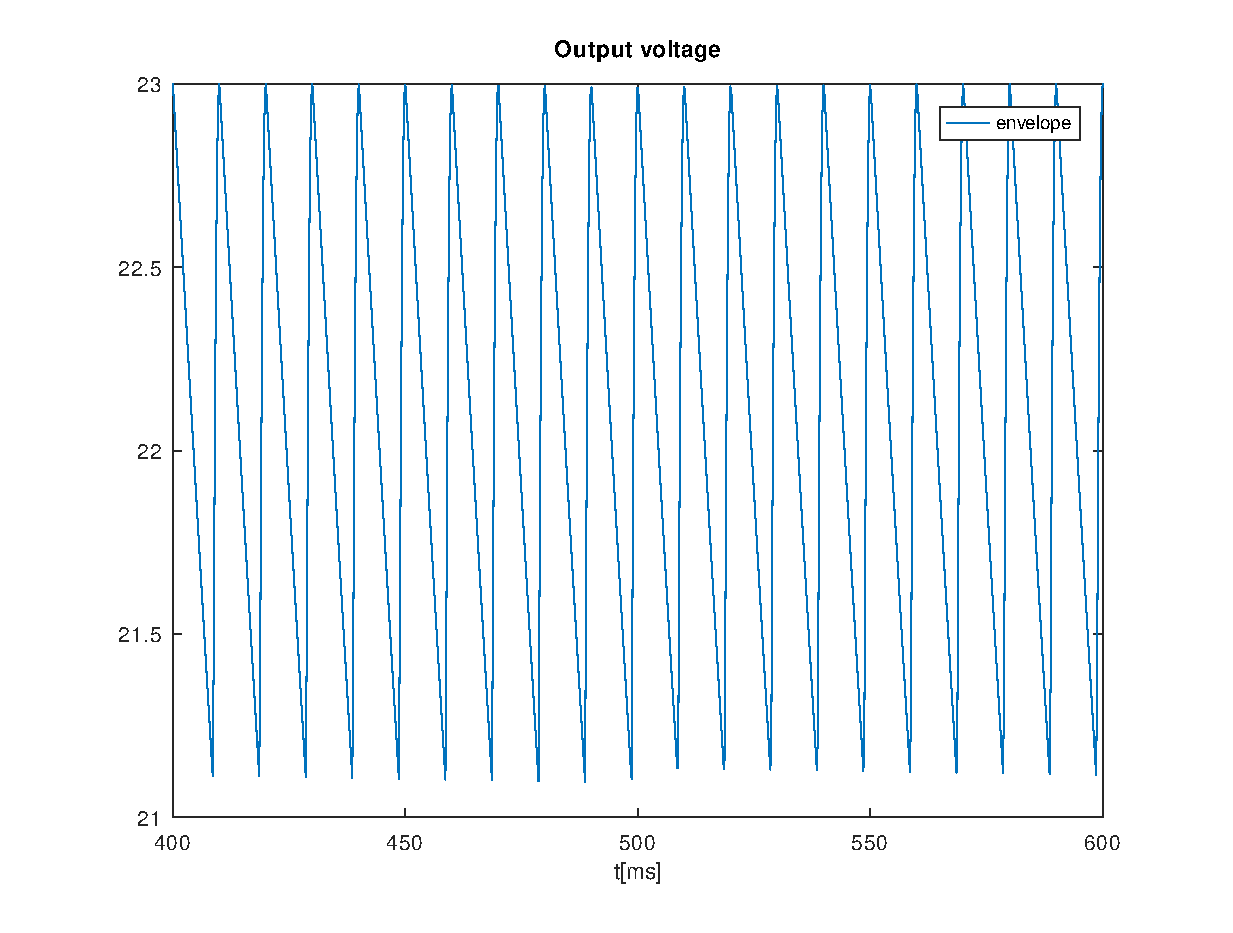
\includegraphics[width=0.6\linewidth]{vOenv_vOr.eps}
\caption{vO Envelope Detector}
\label{fig:vOenv}
\end{figure}

\begin{table}[h]
  \centering
  \begin{tabular}{|l|r|}
    \hline    
    {\bf Name} & {\bf Value [V]} \\ \hline
    \input{../mat/Envelope_tab}
  \end{tabular}
  \caption{Envelope Detector}
  \label{tab:Envelope}
\end{table}
\FloatBarrier


\subsection{Voltage Regulator Output Prediction}
\label{vr}

The theoretical calculations for the Voltage Regulator circuit were based on an incremental model defined by the following equations.

\begin{equation}
v_S=V_S+v_s , v_O=V_O+v_o , V_O=nV_{on} , V_S>nV_{on}
\label{eq:kvl7}
\end{equation}

\begin{equation}
v_o=\frac{nr_d}{nr_d+R})v_s
\label{eq:kvl8}
\end{equation}

The incremental diode resistance is given by

\begin{equation}
\frac{\eta V_T}{I_Se^{\frac{V_D}{\eta V_T}}}
\label{eq:kvl9}
\end{equation}


\begin{figure}[h] \centering
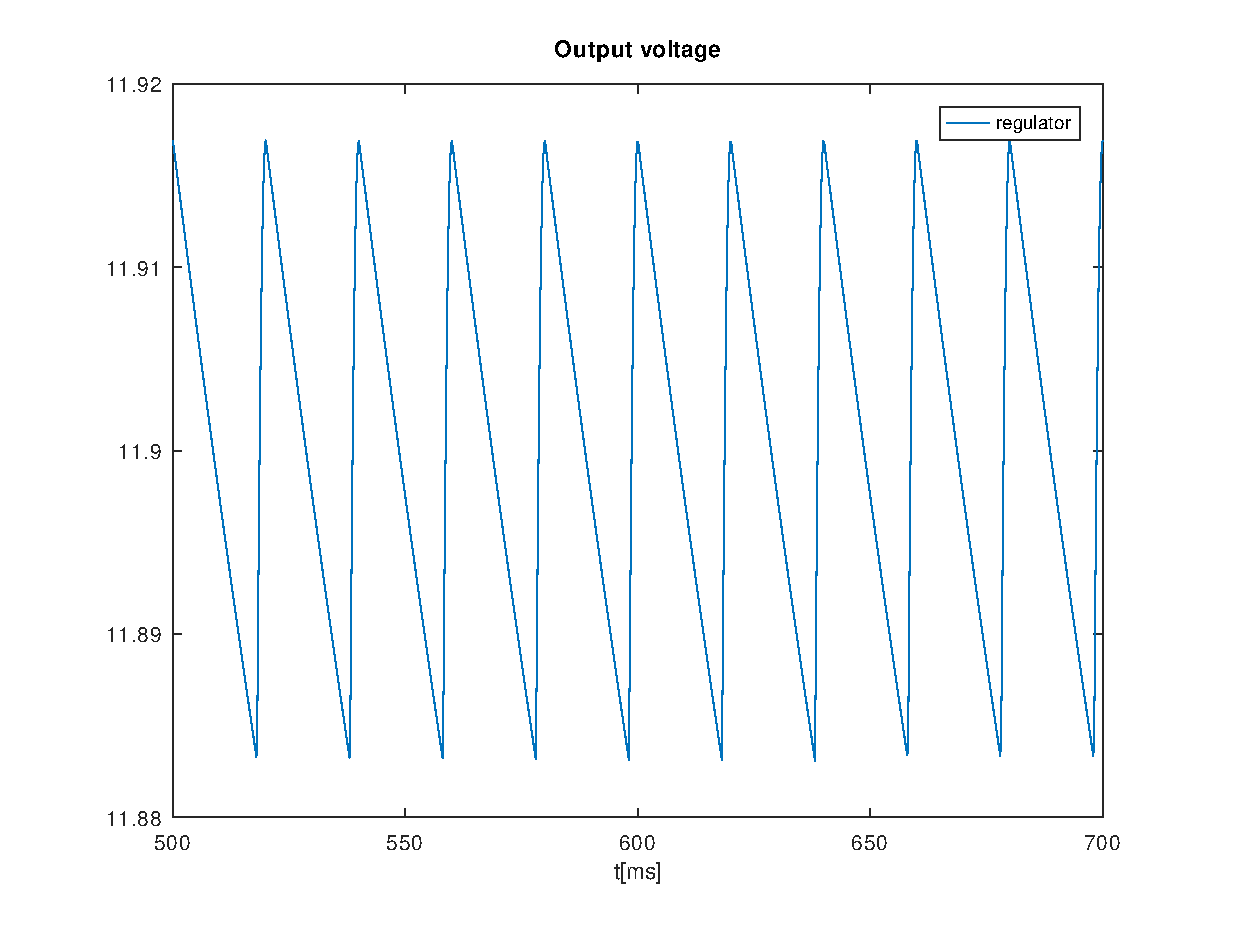
\includegraphics[width=0.6\linewidth]{vOreg.eps}
\caption{vO Voltage Regulator}
\label{fig:vOreg}
\end{figure}


\begin{figure}[h] \centering
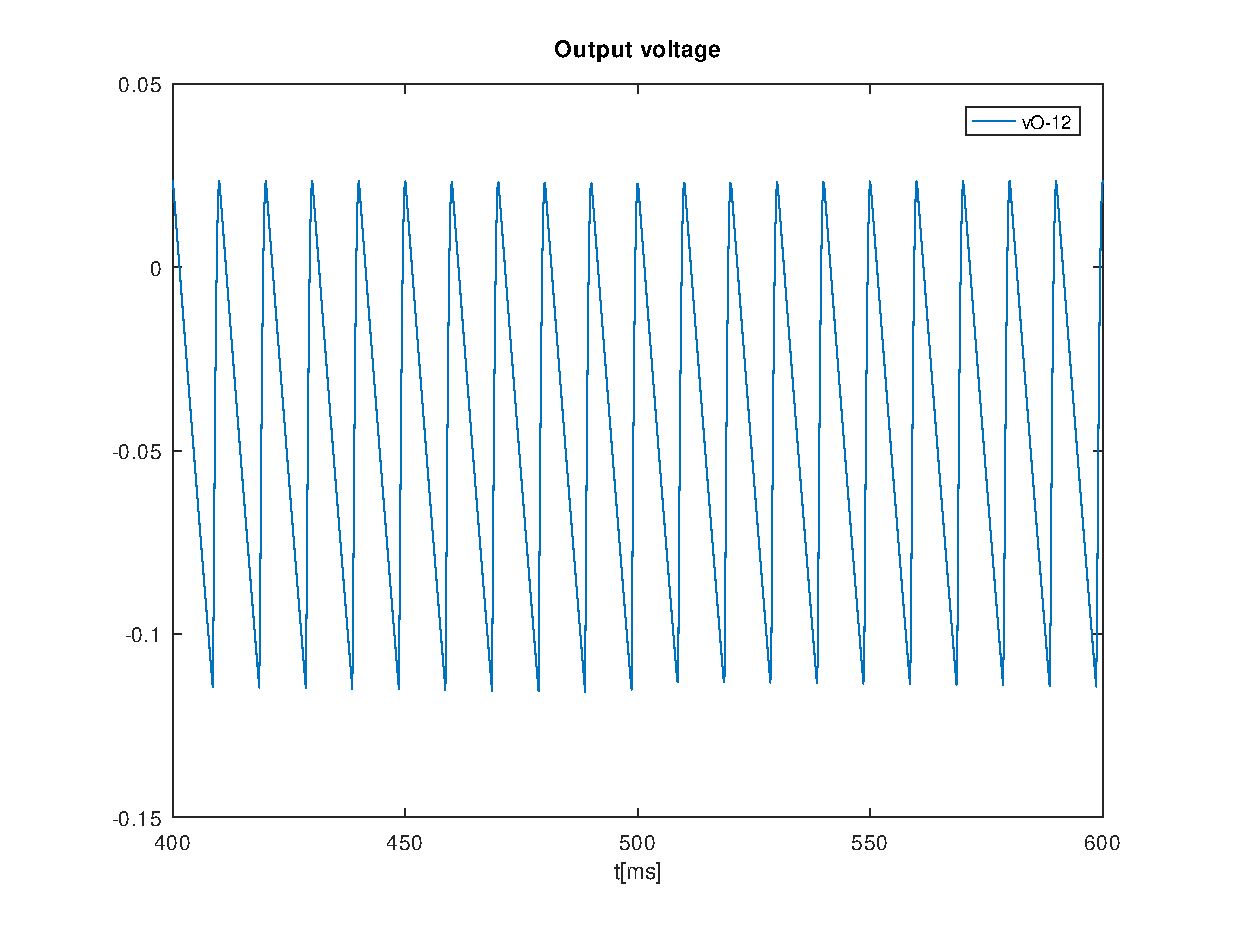
\includegraphics[width=0.6\linewidth]{vO-12.eps}
\caption{vO Voltage Regulator - 12}
\label{fig:vO-12}
\end{figure}


\begin{table}[h]
  \centering
  \begin{tabular}{|l|r|}
    \hline    
    {\bf Name} & {\bf Value [V]} \\ \hline
    \input{../mat/Regulator_tab}
  \end{tabular}
  \caption{Voltage Regulator}
  \label{tab:Regulator}
\end{table}
\FloatBarrier

\subsection{Cost and Merit}
\label{cm}


\begin{table}[h]
  \centering
  \begin{tabular}{|l|r|}
    \hline    
    {\bf Name} & {\bf Value [V]} \\ \hline
    \input{../mat/Merit_tab}
  \end{tabular}
  \caption{Cost and Merit}
  \label{tab:Merit}
\end{table}
\FloatBarrier






